\section{Magnon scattering}\label{sec:14.1}

A dark-matter particle of \SI{1}{MeV} that couples to the spin of the electron can transfer up to \SI{5.3}{keV} of momentum, twice the distance from $\Gamma$ to the ordering wavevector of NiO. It can therefore create a magnon anywhere in the zone, and \cref{sec:7.1} showed that the weight of that magnon depends strongly on where it lands: an antiferromagnet suppresses magnons near $\Gamma$ and enhances them near the ordering wavevector. Here we turn those weights into a rate, from the lightest mass that can emit a magnon above a few meV to masses where the magnetic form factor cuts it off, and we estimate the first correction in $1/|\vect{S}|$.

\subsection{One-magnon response of an antiferromagnet}

Every coupling to the electron spin in \cref{tab:8-operators}, from the contact interaction $\mathcal{O}_4 = \vect{S}_\chi\cdot\vect{S}_e$ to the velocity-dependent $\mathcal{O}_{12}$--$\mathcal{O}_{15}$, reaches the electrons through the spin row $\vect{s}_e(\vect{q})$ of \cref{eq:8.1-rows}, together with the spin current for some of them. In a magnetic insulator the spin density lives on the open shells of the ions, and \cref{eq:7.1-Fmag} replaces $\vect{s}_e(\vect{q})$ by $F^{\mathrm{mag}}(q)\sum_j\ee^{\ii\vect{q}\cdot\vect{r}_j}\vect{S}_j$, a sum over the ionic spins weighted by the magnetic form factor. We take ions whose orbital moment is quenched, as for Ni$^{2+}$; ions with an orbital moment add an orbital row (\cref{app:C.19}, \cref{sec:14.3}). At linear spin-wave order the transverse components $S^\pm$ are linear in the magnon operators and create one magnon, while $S^z$ is quadratic and creates two. The density row creates no magnon at all with the nuclei clamped, so the density--spin blocks of $S_{ab}$ vanish on one-magnon final states.

For the ferromagnet the one-magnon response is \cref{eq:7.1-Sfm}. For the antiferromagnet we need the matrix elements of $S^\pm(\vect{q})$ at any $\vect{q}$, not only near $\Gamma$ and near the ordering wavevector. \Cref{app:D.38} computes them from the operators of \cref{app:D.19}. A momentum transfer outside the zone of one sublattice is reduced by a reciprocal-lattice vector $\vect{G}$ of that sublattice, and the sites of sublattice B, displaced from those of A by $\vect{\delta}_0$, pick up the phase $\ee^{\ii\vect{G}\cdot\vect{\delta}_0} = \pm1$. That phase decides whether the two sublattices add in phase or against each other. Since $J^{\mathrm{ex}}_{\mathrm{AB}}(\vect{q})$ changes sign under a reciprocal vector of the sublattice that maps A onto B, the phase is carried automatically if the coefficients $A_{\vect{k}}$ and $B_{\vect{k}}$ of \cref{eq:7.1-Hk} are evaluated at the full momentum transfer rather than at its reduced value. The two degenerate magnons, one created by $S^-$ and one by $S^+$, precess in opposite senses and have equal weight. Inserted into \cref{eq:4.2-Sab}, their circular polarizations add to a linear one:
\begin{keyresult}[One-magnon spin response of a two-sublattice antiferromagnet]
\begin{equation}
  S_{ab}(\vect{q},\omega) = \frac{\pi|\vect{S}|}{\Omega_{\mathrm{ion}}}\,|F^{\mathrm{mag}}(q)|^2\,w^{\mathrm{M}}_{\vect{q}}\,\bigl(\delta_{ab} - \hat z_a\hat z_b\bigr)\,\delta\bigl(\omega - \omega^{\mathrm{M}}_{\vect{q}}\bigr), \qquad
  w^{\mathrm{M}}_{\vect{q}} = \frac{|\vect{S}|\,(A_{\vect{q}} - B_{\vect{q}})}{\omega^{\mathrm{M}}_{\vect{q}}} ,
  \label{eq:14.1-Safm}
\end{equation}
for $T = 0$, $\omega > 0$ and moments along $\pm\hat{\vect{z}}$, with $\Omega_{\mathrm{ion}}$ the volume per magnetic ion (for NiO the volume of the chemical primitive cell), $\omega^{\mathrm{M}}_{\vect{q}}$ of \cref{eq:7.1-afm}, and $A_{\vect{q}}$, $B_{\vect{q}}$ of \cref{eq:7.1-Hk} at the momentum transfer $\vect{q}$ itself.
\end{keyresult}
\noindent Compared to the ferromagnet of \cref{eq:7.1-Sfm}, two things change. The antisymmetric part $\ii\epsilon_{abc}\hat z_c$ is gone, because the antiferromagnet offers both senses of precession; it absorbs a transverse probe of either circular polarization. The weight is no longer one: $w^{\mathrm{M}}_{\vect{q}}$ is the factor $(u^{\mathrm{M}} \mp v^{\mathrm{M}})^2$ of \cref{eq:7.1-weights}, now written so that it holds at every $\vect{q}$ (\cref{eq:D.38-weight}). The matrix in brackets has eigenvalues $1$, $1$ and $0$, so \cref{eq:14.1-Safm} is positive semidefinite as long as $w^{\mathrm{M}}_{\vect{q}} \ge 0$, which is the stability condition $A_{\vect{q}} \ge |B_{\vect{q}}|$ of \cref{sec:7.1}.

The weight has a simple form near the two points where the magnon energy vanishes. Write $(\omega^{\mathrm{M}}_{\vect{q}})^2 = |\vect{S}|^2(A_{\vect{q}} - B_{\vect{q}})(A_{\vect{q}} + B_{\vect{q}})$. Near $\Gamma$ the sum $A + B$ tends to $2J^{\mathrm{ex}}_{\mathrm{AB}}(0)$, so
\begin{equation*}
  w^{\mathrm{M}}_{\vect{q}} \simeq \frac{\omega^{\mathrm{M}}_{\vect{q}}}{2|\vect{S}|J^{\mathrm{ex}}_{\mathrm{AB}}(0)} \quad (\vect{q} \to 0), \qquad
  w^{\mathrm{M}}_{\vect{q}} \simeq \frac{2|\vect{S}|J^{\mathrm{ex}}_{\mathrm{AB}}(0)}{\omega^{\mathrm{M}}_{\vect{q}}} \quad (\vect{q} \to \vect{Q}_{\mathrm{AF}}) ,
\end{equation*}
where near the ordering wavevector $\vect{Q}_{\mathrm{AF}}$, $(\pi/a)(1,1,1)$ in NiO, $B_{\vect{q}} \to -J^{\mathrm{ex}}_{\mathrm{AB}}(0)$ and the difference $A - B$ takes the large value instead. The scale is the exchange energy $2|\vect{S}|J^{\mathrm{ex}}_{\mathrm{AB}}(0) = 12|\vect{S}|(J_1 + J_2) = \SI{211.7}{meV}$ for NiO. A magnon of \SI{5}{meV} near $\Gamma$ carries $w^{\mathrm{M}} = 0.024$, a magnon of the same energy near $\vect{Q}_{\mathrm{AF}}$ carries 42, and a ferromagnet would give 1 to both. Physically, a long-wavelength transverse probe tries to tilt the two sublattices the same way, against the full exchange field. A probe that alternates in sign from one $(111)$ plane to the next tilts them in opposite directions, which rotates the Néel order as a whole and costs almost nothing. Evaluated within \SI{0.01}{\angstrom^{-1}} of either point, \cref{eq:14.1-Safm} agrees with these forms to \SI{0.02}{\percent}.

The exchange constants that fix $A_{\vect{q}}$, $B_{\vect{q}}$ and $\omega^{\mathrm{M}}_{\vect{q}}$ come, for NiO, from the neutron fit of \cref{eq:7.1-NiO}. For a magnet without such data they are computed in DFT~$+\,U$ by the energy-mapping, spin-spiral or Green's-function routes of \cref{app:E.9}, together with the single-ion anisotropies that open the gaps. \Cref{app:E.20-magnet} specifies these calculations for yttrium iron garnet (YIG), NiO, MnO, Cr$_2$O$_3$ and NiPS$_3$. The spread of the computed $J_2$ of NiO, 11 to \SI{27}{meV} (\cref{sec:7.1}), scales $\omega^{\mathrm{M}}$ but leaves $w^{\mathrm{M}}_{\vect{q}}$ unchanged, since the weight depends only on ratios of exchange constants. A ferrimagnet such as YIG, with 20 magnetic ions per primitive cell, needs the multi-sublattice Bogoliubov transformation in place of \cref{eq:14.1-Safm}.

\subsection{Rate formula and mass edge}

The rate follows from \cref{eq:8.2-spectrum} with $S_{ab}$ of \cref{eq:14.1-Safm} in the spin block. Since the response is proportional to $\delta_{ab} - \hat z_a\hat z_b$, the contraction picks out the part of the dark-matter tensor transverse to the moments,
\begin{equation}
  \sum_{a,b}\mathfrak{D}_{ab}S_{ab}(\vect{q},\omega) = \frac{\pi|\vect{S}|}{\Omega_{\mathrm{ion}}}\,|F^{\mathrm{mag}}(q)|^2\,w^{\mathrm{M}}_{\vect{q}}\,\bigl[\Tr\mathfrak{D} - \hat{\vect{z}}\cdot\mathfrak{D}\cdot\hat{\vect{z}}\bigr]\,\delta\bigl(\omega - \omega^{\mathrm{M}}_{\vect{q}}\bigr) ,
  \label{eq:14.1-contract}
\end{equation}
with $\mathfrak{D}_{ab}$ of \cref{eq:8.1-D} for the spin rows. For $\mathcal{O}_4$, the spin-dependent contact interaction, $\mathfrak{D}_{ab} = |c_4^{(e)}|^2\delta_{ab}/4$ for dark matter of spin $\frac12$, the bracket is $|c_4^{(e)}|^2/2$, and the rate does not depend on the direction of the moments. For $\mathcal{O}_6$, whose tensor is proportional to $q_aq_b$, the bracket is proportional to $1 - (\hat{\vect{q}}\cdot\hat{\vect{z}})^2$. Only the component of the momentum transfer perpendicular to the moments then creates a magnon, and the rate of a fixed crystal changes as the Earth turns the wind relative to the moments.

We present rates for $\mathcal{O}_4$ with a heavy mediator, $c_4^{(e)}$ independent of $q$. The reference cross-section is that of the same operator on a free electron, $\sigmae = \mu_{\chi e}^2\langle|\tilde V|^2\rangle/\pi$ as in \cref{sec:1.4}, with the average over both spins. Since $\langle|\vect{S}_\chi\cdot\vect{S}_e|^2\rangle = \sum_{a,b}\Tr(S^a_\chi S^b_\chi)\Tr(S^a_eS^b_e)/4 = 3/16$,
\begin{equation}
  \sigmae = \frac{3\mu_{\chi e}^2|c_4^{(e)}|^2}{16\pi} ,
  \label{eq:14.1-sigma}
\end{equation}
the definition of Trickle, Zhang and Zurek~\cite[Eq.~(11)]{trickle2020detecting} for this operator. The response depends on the direction of $\vect{q}$ through $w^{\mathrm{M}}_{\vect{q}}$ and $\omega^{\mathrm{M}}_{\vect{q}}$, and the full velocity kernel of \cref{app:A.8} gives the daily modulation of a fixed crystal. Averaged over the orientations of the crystal relative to the wind, the kernel is $\eta(\vmin)/2q$ per $\dd^3q/(2\pi)^3$ (\cref{eq:A.8-eta}). The rate per unit target mass above a threshold $\omega_{\mathrm{th}}$ is then
\begin{equation}
  \mathcal{R}(\omega_{\mathrm{th}}) = \frac{2\rho_\chi\sigmae|\vect{S}|}{3\,\mchi\rho_T\,\mu_{\chi e}^2\,\Omega_{\mathrm{ion}}}\int_0^{\infty}\dd q\,q\,\Bigl\langle|F^{\mathrm{mag}}(q)|^2\,w^{\mathrm{M}}_{\vect{q}}\,\eta\bigl(\vmin(q,\omega^{\mathrm{M}}_{\vect{q}})\bigr)\,\Theta\bigl(\omega^{\mathrm{M}}_{\vect{q}} - \omega_{\mathrm{th}}\bigr)\Bigr\rangle_{\hat{\vect{q}}} ,
  \label{eq:14.1-rate}
\end{equation}
with $\langle\cdots\rangle_{\hat{\vect{q}}}$ the average over the directions of $\vect{q}$ at fixed $q$ and $\vmin = \omega/q + q/2\mchi$ from \cref{eq:1.3-vmin}. The numerical factor collects $\pi|c_4^{(e)}|^2/2$ from \cref{eq:14.1-contract}, $16\pi\sigmae/3\mu_{\chi e}^2$ from \cref{eq:14.1-sigma}, and $1/4\pi^2$ from the angular integral. At $F^{\mathrm{mag}} = 1$, \cref{eq:14.1-rate} is the orientation average of the one-magnon rate of Trickle, Zhang and Zurek~\cite[Eqs.~(5)--(10)]{trickle2020detecting}, which their later work extends to all the operators of \cref{tab:8-operators}~\cite[Eqs.~(34) and~(38)]{trickle2022effective}. For one sublattice, $w^{\mathrm{M}} = 1$ and the bracket of the ferromagnet replaces that of \cref{eq:14.1-contract}; the result is their ferromagnetic rate~\cite[Eq.~(12)]{trickle2020detecting} with the spin density $|\vect{S}|/\Omega_{\mathrm{ion}}$.

The lightest mass that reaches a threshold follows from the linear dispersion near the gapless points, $\omega^{\mathrm{M}} \simeq c_{\mathrm{M}}|\vect{q} - \vect{k}_0|$ with $\vect{k}_0$ either $0$ or $\vect{Q}_{\mathrm{AF}}$ and $c_{\mathrm{M}}$ the magnon velocity. The momentum transfer from light dark matter is small, so only the region near $\Gamma$ counts. A magnon of momentum $q$ can be emitted if $c_{\mathrm{M}}q \le qv - q^2/2\mchi$, that is, for $q \le 2\mchi(v - c_{\mathrm{M}})$, and it lies above threshold for $q \ge \omega_{\mathrm{th}}/c_{\mathrm{M}}$. Both hold at the fastest speed when
\begin{equation}
  \mchi \ge \frac{\omega_{\mathrm{th}}}{2c_{\mathrm{M}}(v_{\mathrm{max}} - c_{\mathrm{M}})} ,
  \label{eq:14.1-mmin}
\end{equation}
the magnon analog of the acoustic edge of \cref{sec:11.1}. The speed $c_{\mathrm{M}} = 1.39\times10^{-4}$ of \cref{we:7-nio} is that of $J_2$ alone. With $J_1$ added, the model of \cref{fig:14-nio-rate} has speeds from $1.29\times10^{-4}$ to $1.36\times10^{-4}$ depending on direction, and the fastest puts the edge for $\omega_{\mathrm{th}} = \SI{5}{meV}$ at \SI{7.3}{keV}. Near the edge, however, the weight is $w^{\mathrm{M}} \simeq \omega_{\mathrm{th}}/2|\vect{S}|J^{\mathrm{ex}}_{\mathrm{AB}}(0) = 0.024$, and the antiferromagnet starts about forty times below a ferromagnet with the same magnon velocity.

\subsection{Zero-point spin reduction}

Linear spin-wave theory is the leading order of an expansion in $1/|\vect{S}|$, and for Ni$^{2+}$, with $|\vect{S}| = 1$, the expansion parameter $1/(2|\vect{S}|)$ is one half. The size of the first correction to \cref{eq:14.1-rate} follows from a sum rule. Each ionic spin has a fixed length, $\vect{S}_i^2 = |\vect{S}|(|\vect{S}| + 1)$, and the equal-time correlations of one site split that total into three parts. The static moment $\langle S^z_i\rangle^2$ scatters only elastically, into Bragg peaks. The transverse fluctuations $W_\perp = \langle S^x_iS^x_i + S^y_iS^y_i\rangle$ are, at linear order, all one-magnon weight. The longitudinal fluctuations $W_\parallel = \langle(S^z_i)^2\rangle - \langle S^z_i\rangle^2$ create magnon pairs. Each weight is the integral of the corresponding block of $S_{ab}$ over $\omega$ and over the zone. Together they fix how the spectral weight that a spin coupling can reach is divided between the one-magnon line, the two-magnon continuum and the elastic peaks, which deposit no energy.

In the Néel state the transverse fluctuations would be $|\vect{S}|$ and the longitudinal ones zero. The true ground state is not the Néel state. The pair term of \cref{eq:7.1-Hk} mixes in states with a deviation on each sublattice, and each mode leaves the zero-point deviation $(v^{\mathrm{M}}_{\vect{k}})^2$ on every site (\cref{sec:7.1}). \Cref{app:D.38} evaluates the three weights in this ground state, the longitudinal one by Wick's theorem:
\begin{keyresult}[Spin weights at linear spin-wave order]
\begin{equation}
  \begin{gathered}
  \Delta S = \frac{1}{N_{\mathrm{s}}}\sum_{\vect{k}}\bigl(v^{\mathrm{M}}_{\vect{k}}\bigr)^2, \qquad
  W_\perp = |\vect{S}|\,(1 + 2\Delta S), \qquad
  W_\parallel = \Delta S\,(1 + \Delta S), \\
  \frac{W_\parallel}{W_\perp} = \frac{\Delta S\,(1 + \Delta S)}{|\vect{S}|\,(1 + 2\Delta S)} ,
  \end{gathered}
  \label{eq:14.1-ratio}
\end{equation}
with the sum over the zone of one sublattice and the ordered moment $\langle S^z_i\rangle = |\vect{S}| - \Delta S$.
\end{keyresult}
\noindent The zero-point spin reduction $\Delta S$ depends on the lattice and on ratios of exchange constants, not on $|\vect{S}|$, so the ratio falls as $1/|\vect{S}|$ with a coefficient fixed by the lattice. For a ferromagnet $v^{\mathrm{M}}_{\vect{k}} = 0$, and both $\Delta S$ and $W_\parallel$ vanish: the fully polarized state is exact, and a longitudinal probe finds nothing to excite. For an antiferromagnet the zone average of the weight $w^{\mathrm{M}}_{\vect{q}}$ of \cref{eq:14.1-Safm} is $1 + 2\Delta S$, which is the same statement as $W_\perp$, and gives a check of any numerical evaluation of the one-magnon response.

The three weights violate the sum rule. Added up, $W_\perp + W_\parallel + \langle S^z_i\rangle^2$ exceeds $|\vect{S}|(|\vect{S}| + 1)$ by $\Delta S(1 + 2\Delta S)$, because linear spin-wave theory replaces the square roots of the Holstein--Primakoff transformation \cref{eq:7.1-HP} by their value at zero deviation. Holding the ordered moment and $W_\parallel$ at the values of \cref{eq:14.1-ratio}, the sum rule requires the transverse weight $(|\vect{S}| - \Delta S)(1 + 2\Delta S)$, and \cref{app:D.38} shows that the full square roots, evaluated in the same ground state, give exactly this value. At this order, with $\langle S^z_i\rangle$ and $W_\parallel$ held at their linear spin-wave values, the one-magnon weight of linear spin-wave theory is too large by the fraction $\Delta S/|\vect{S}|$. This is an estimate of the leading correction, not a bound. The corrected transverse operator also creates three magnons, which lowers the one-magnon part further; however, the change of the ground state at the same order, which moves $\langle S^z_i\rangle$ and $W_\parallel$ as well, is not part of the estimate. The one-magnon and two-magnon weights together, $(|\vect{S}| - \Delta S)(1 + 2\Delta S) + \Delta S(1 + \Delta S) = |\vect{S}|(1 + 2\Delta S) - \Delta S^2$, agree with the linear spin-wave one-magnon weight up to $\Delta S^2$. The first correction does not remove weight; it moves the fraction $\Delta S/|\vect{S}|$ of it from the one-magnon line into the two-magnon continuum, which lies at other energies for the same momentum transfer (\cref{sec:14.2}).

\begin{workedexample}{The zero-point spin reduction of NiO}\label{we:14-nio}
For the type-II order of NiO with the exchange constants \cref{eq:7.1-NiO}, $(v^{\mathrm{M}}_{\vect{k}})^2 = \frac12[A_{\vect{k}}(A_{\vect{k}}^2 - B_{\vect{k}}^2)^{-1/2} - 1]$ with $A_{\vect{k}}$ and $B_{\vect{k}}$ of \cref{eq:7.1-Hk}. We average it over a $100^3$ grid of the cube of side $4\pi/a$, the period of the reciprocal lattice of the nickel ions along each cube axis, which holds every wavevector of the zone twice, and find
\begin{equation*}
  \Delta S = 0.0784 .
\end{equation*}
The grid avoids the gapless points at $\Gamma$ and $\vect{Q}_{\mathrm{AF}}$, where $(v^{\mathrm{M}})^2$ diverges as the inverse distance; this singularity is integrable. The sum changes by $1.1\times10^{-4}$ from $60^3$ to $80^3$ points and by $5\times10^{-5}$ from $80^3$ to $100^3$, as the inverse square of the grid size, and extrapolates to 0.0785. With $J_1 = 0$ it is $0.0783$. The reason is that the next-nearest neighbors at $\pm a\hat{\vect{x}}$, $\pm a\hat{\vect{y}}$, $\pm a\hat{\vect{z}}$ link the fcc lattice into four interpenetrating simple-cubic lattices of side $a$, each a Néel antiferromagnet. Their zero-point reduction is Anderson's 0.078 for the simple-cubic antiferromagnet~\cite{anderson1952approximate}, and the weak $J_1$ barely changes it.

With $|\vect{S}| = 1$, the ordered moment is $|\vect{S}| - \Delta S = 0.9216$ of its classical value, and \cref{eq:14.1-ratio} gives
\begin{equation*}
  W_\perp = 1.157, \qquad W_\parallel = 0.0846, \qquad \frac{W_\parallel}{W_\perp} = \frac{0.0784 \times 1.0784}{1 \times 1.1569} = 0.0731 .
\end{equation*}
The sum rule requires $W_\perp = 0.9216 \times 1.1569 = 1.066$: at this order the one-magnon weight of linear spin-wave theory, and with it the rate \cref{eq:14.1-rate}, is high by about $\Delta S/|\vect{S}| = \SI{7.8}{\percent}$. The two-magnon continuum holds \SI{7.3}{\percent} of the linear spin-wave one-magnon weight, and the total, one-magnon plus two-magnon, is $0.995$ of it. The ratio $\Delta S/|\vect{S}| = 0.078$ is six times smaller than the expansion parameter $1/(2|\vect{S}|) = 0.5$. In three dimensions the zero-point motion of the spin waves is small, and the expansion in $1/|\vect{S}|$ converges faster than its parameter suggests.
\end{workedexample}

\Cref{lim:14.1a} sets the literature rate against these weights as $|\vect{S}|$ varies at the fixed lattice and exchange ratios of NiO, where $\Delta S = 0.078$ throughout.
\begin{limitbox}[One-magnon rate at linear spin-wave order][lim:14.1a]
$\varGamma(\vect{v}) = \int\frac{\dd^3q}{(2\pi)^3}\sum_{a,b}\mathfrak{D}_{ab}S_{ab}(\vect{q},\omega_{\vect{q}})$ with the one-magnon response \cref{eq:14.1-Safm} at $F^{\mathrm{mag}} = 1$, spectral weight $W_\perp = |\vect{S}|(1 + 2\Delta S)$ per ion~\cites[Eqs.~(5)--(12)]{trickle2020detecting}[Eq.~(38)]{trickle2022effective}.
\par\smallskip
{\centering
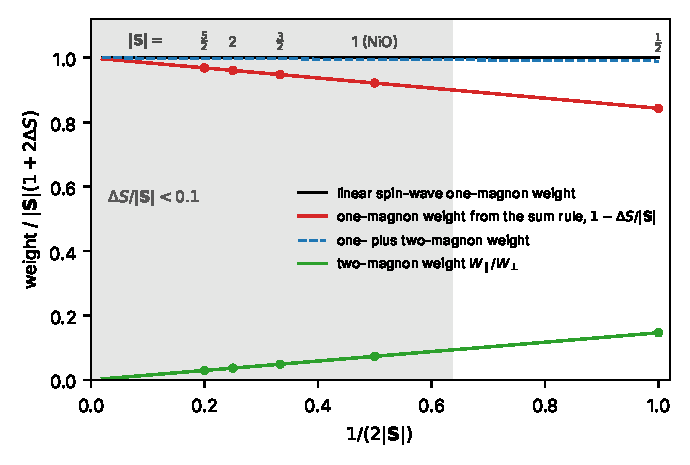
\includegraphics[width=0.92\linewidth]{figures/ch14/limit14_1a.pdf}
\captionof{figure}{Spectral weights of the spin of one magnetic ion against the expansion parameter $1/(2|\vect{S}|)$, in units of the one-magnon weight of linear spin-wave theory, $|\vect{S}|(1 + 2\Delta S)$, which the literature rate contains (black line). Red: the one-magnon weight that the sum rule $\vect{S}^2 = |\vect{S}|(|\vect{S}| + 1)$ requires, $1 - \Delta S/|\vect{S}|$. Green: the two-magnon weight $W_\parallel/W_\perp$ of \cref{eq:14.1-ratio}. Dashed: one- plus two-magnon weight, $1 - \Delta S^2/[|\vect{S}|(1 + 2\Delta S)]$. Lattice and exchange ratios of NiO (type-II order, $J_1/J_2 = -0.072$), zero-point reduction $\Delta S = 0.078$ from a $100^3$ grid; points at $|\vect{S}| = \frac12$, 1 (NiO), $\frac32$, 2 and $\frac52$. Gray: $\Delta S/|\vect{S}| < 0.1$, which holds for $|\vect{S}| \ge 0.78$.}\label{fig:14-limit-magnon}
\par}
\smallskip
For $|\vect{S}| = \frac12$ the one-magnon line is overcounted by about \SI{16}{\percent} at this order and the two-magnon weight reaches \SI{15}{\percent}, and the magnon interactions of the next order, which shift and broaden the magnons, are no longer small.
\end{limitbox}

For Mn$^{2+}$ and Fe$^{3+}$, with $|\vect{S}| = \frac52$, the same lattice gives a defect of \SI{3.1}{\percent} and a two-magnon weight of \SI{2.9}{\percent}. The rates of this section use the exchange fitted to the measured magnons, so the shift of the magnon energies by the quartic terms of the Holstein--Primakoff expansion is already absorbed into $J_1$ and $J_2$ (\cref{we:7-nio}). The division of weight in \cref{fig:14-limit-magnon} is not.

\subsection{The one-magnon rate of NiO}

The inputs for NiO are those of \cref{sec:7.1}: the exchange constants \cref{eq:7.1-NiO}, $|\vect{S}| = 1$, and $a = \SI{4.17}{\angstrom}$, so that the volume per nickel ion is $\Omega_{\mathrm{ion}} = a^3/4 = \SI{18.13}{\angstrom^3}$ and the density, from four formula units per cubic cell, is $\rho_T = \SI{6.84}{g.cm^{-3}}$. The form factor of Ni$^{2+}$, whose orbital moment is quenched, is the spin-only $F^{\mathrm{mag}} = \langle j_0(q)\rangle$ of \cref{eq:C.19-spinonly}. We take $\langle j_0\rangle$ from the tabulated fit $A\ee^{-\alpha s^2} + B\ee^{-\beta s^2} + C\ee^{-\gamma s^2} + D$ with $s = q/4\pi$, in \si{\angstrom^{-1}}, and the coefficients $(A, \alpha, B, \beta, C, \gamma, D) = (0.0163, 35.88, 0.3916, 13.22, 0.6052, 4.339, -0.0133)$~\cite[Sect.~4.4.5, Table~4.4.5.2]{anderson2006neutron}. It gives $|F^{\mathrm{mag}}|^2 = 0.84$ at $|\vect{Q}_{\mathrm{AF}}| = \SI{2.6}{keV}$ and 0.49 at \SI{5.3}{keV}, the largest momentum transfer of a \SI{1}{MeV} particle.

Two limits fix the shape of the rate before any integral is done. At the light end, \cref{eq:14.1-mmin} sets the edge, and above it the weight near $\Gamma$ grows in proportion to the magnon energy. At the heavy end, the momentum transfers sweep many zones and the magnon energies, at most \SI{118}{meV}, are negligible against $qv$. Then $\vmin \simeq q/2\mchi$, the direction average of $w^{\mathrm{M}}_{\vect{q}}$ over a shell that crosses many zones tends to its zone average $1 + 2\Delta S$, and $\int\dd q\,q\,\eta(q/2\mchi) = 4\mchi^2\int\dd u\,u\,\eta(u) = 2\mchi^2\langle v\rangle$, with $\langle v\rangle$ the mean speed of the dark matter in the laboratory. \Cref{eq:14.1-rate} at $F^{\mathrm{mag}} = 1$ becomes
\begin{equation}
  \mathcal{R} \simeq \frac{\rho_\chi}{\mchi}\,\frac{\langle v\rangle}{\rho_T\Omega_{\mathrm{ion}}}\,\sigmae\Bigl(\frac{\mchi}{\mu_{\chi e}}\Bigr)^2\,\frac{|\vect{S}|(1 + 2\Delta S)}{3/4} .
  \label{eq:14.1-inc}
\end{equation}
This is the flux of dark matter times the number of ions per unit mass times a cross-section per ion. At large $q$ the magnet looks like a gas of free spins, each with the transverse weight $W_\perp$ in place of the electron's $\frac34$, and with the reduced mass $\mu_{\chi e}$ replaced by $\mchi$ for a heavy target. With $\langle v\rangle = \SI{354}{km/s}$ for the halo of \cref{sec:1.2}, the integral \cref{eq:14.1-rate} at $F^{\mathrm{mag}} = 1$ is 0.96 of \cref{eq:14.1-inc} at \SI{3}{MeV} and 0.989 at \SI{10}{MeV}.

\begin{figure}[tbp]
  \centering
  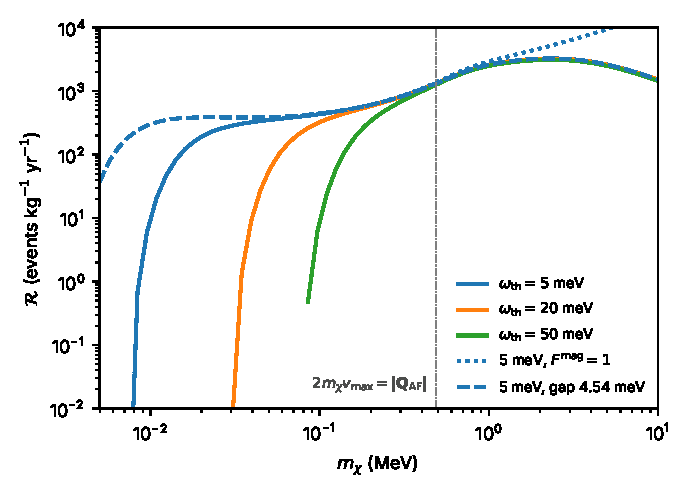
\includegraphics[width=0.75\linewidth]{figures/ch14/fig14_1.pdf}
  \caption{One-magnon rate of NiO per kilogram-year for dark matter with the spin-dependent contact interaction $\mathcal{O}_4 = \vect{S}_\chi\cdot\vect{S}_e$ (heavy mediator) at the reference cross-section $\sigmae = \SI{e-40}{cm^2}$ of \cref{eq:14.1-sigma}, against the dark-matter mass, from \cref{eq:14.1-rate}: $T = 0$, rate averaged over the orientations of the crystal relative to the dark-matter wind, standard halo of \cref{sec:1.2}. Solid: energy thresholds of 5, 20 and \SI{50}{meV}. Model: Heisenberg exchange $J_1 = -\SI{1.37}{meV}$, $J_2 = \SI{19.01}{meV}$ from neutron scattering, $|\vect{S}| = 1$, $a = \SI{4.17}{\angstrom}$, undistorted fcc lattice without anisotropy (gapless), linear spin-wave theory, magnetic form factor of Ni$^{2+}$. Dotted: \SI{5}{meV} threshold without the form factor, $F^{\mathrm{mag}} = 1$. Dashed: \SI{5}{meV} threshold with an easy-axis single-ion anisotropy added to $A_{\vect{k}}$ and chosen to put the zone-center gap at \SI{4.54}{meV}, the zone-center magnon of NiO seen in far-infrared absorption. Vertical line: the mass at which the largest momentum transfer, $2\mchi v_{\mathrm{max}}$, reaches the ordering wavevector, \SI{0.49}{MeV}.}
  \label{fig:14-nio-rate}
\end{figure}

\Cref{fig:14-nio-rate} shows the full integral. At a threshold of \SI{5}{meV} the rate rises from the edge, at \SI{7.4}{keV} on the mass grid of the figure, to 10 events per kilogram-year at \SI{10}{keV}, 280 at \SI{30}{keV} and 430 at \SI{100}{keV}, for $\sigmae = \SI{e-40}{cm^2}$. At \SI{100}{keV} all of it comes from momentum transfers within half the distance to $\vect{Q}_{\mathrm{AF}}$, where the weight is suppressed. Once the momentum transfer reaches the ordering wavevector the enhanced magnons there take over, and at \SI{1}{MeV}, where the rate is $2.6\times10^3$, only \SI{19}{\percent} of it comes from the region near $\Gamma$. The rate peaks at $3.2\times10^3$ near \SI{3}{MeV} and then falls, because the form factor removes the momentum transfers beyond the inverse radius of the $3d$ shell. It costs a factor 0.89 at \SI{1}{MeV}, and a factor 11.4 against $F^{\mathrm{mag}} = 1$ at \SI{10}{MeV}, where the rate is $1.5\times10^3$. The threshold matters only for the lightest masses. Above \SI{0.3}{MeV} the rates at 5, 20 and \SI{50}{meV} differ by less than \SI{20}{\percent}, since most of the rate then comes from magnons above \SI{50}{meV}. Below, the higher thresholds push the edge up to \SI{30}{keV} and \SI{85}{keV}. The second is later than \cref{eq:14.1-mmin} gives for \SI{50}{meV}, because the dispersion bends over below its maximum.

Near its gap the rate depends on what the Heisenberg model leaves out. Magnetic anisotropy, which \cref{sec:7.1} neglected, lifts the Goldstone modes at $\Gamma$ and $\vect{Q}_{\mathrm{AF}}$ to energies below \SI{5}{meV}. The undistorted $J_1$--$J_2$ model also has a third, accidental zero at $\mathrm{X} = (2\pi/a)(1,0,0)$, where $A_{\vect{k}} = B_{\vect{k}} = 6J_2 - 2J_1$; the weight vanishes there, and the rhombohedral distortion of the real crystal lifts it. Far-infrared absorption places a zone-center magnon of NiO at \SI{4.54}{meV}, the value used by Hutchings and Samuelsen~\cite{hutchings1972measurement} and quoted by dos Santos and collaborators~\cite[Sect.~III]{dossantos2026comparative}. We add an easy-axis term $K$ to $A_{\vect{k}}$, which keeps the form of \cref{eq:7.1-Hk}, and choose $K = \SI{0.0973}{meV}$ so that $|\vect{S}|[(A_0 + K)^2 - A_0^2]^{1/2} = \SI{4.54}{meV}$. With a \SI{5}{meV} threshold the rate then grows by a factor of 29 at \SI{10}{keV} and 1.35 at \SI{30}{keV}, and changes by less than \SI{3}{\percent} above \SI{100}{keV}. The gap puts magnons just above threshold at vanishing momentum, where the kinematics is easiest, and their weight $K^{1/2}/(2A_0)^{1/2}$ is set by the anisotropy. For dark matter lighter than about \SI{50}{keV}, the rate of NiO near its gap is set by its anisotropy. The real anisotropy is biaxial: it keeps the moments in the $(111)$ planes (\cref{fig:7-nio}) and gaps the two branches differently, so that only one of them reaches \SI{4.54}{meV} while the in-plane branch lies near \SI{0.6}{meV}. The one-constant model gaps both at \SI{4.54}{meV}, and the factor 29 is an upper value. The anisotropy enters through the uniform modes of \cref{sec:14.3} and the anisotropy constants of \cref{app:E.20-magnet}. Temperature adds thermal magnons with occupation $\ee^{-\omega^{\mathrm{M}}/T}$; at the gap of \SI{4.54}{meV} the exponent is $-5\times10^3$ at \SI{10}{mK} and $-53$ at \SI{1}{K}, and the zero-temperature response holds at any cryogenic operating point.
